\chapter[Analysis]{Analysis} \label{cha:Analysis}
In this chapter various test setups will be discussed for the purpose of making quantifiable measurements of the amplifier, effects of the output filters parasitic elements on the control loop among others.

\section{Hysteresis window of modulator (Simulation)}

\begin{figure}[htbp]
	\centering
	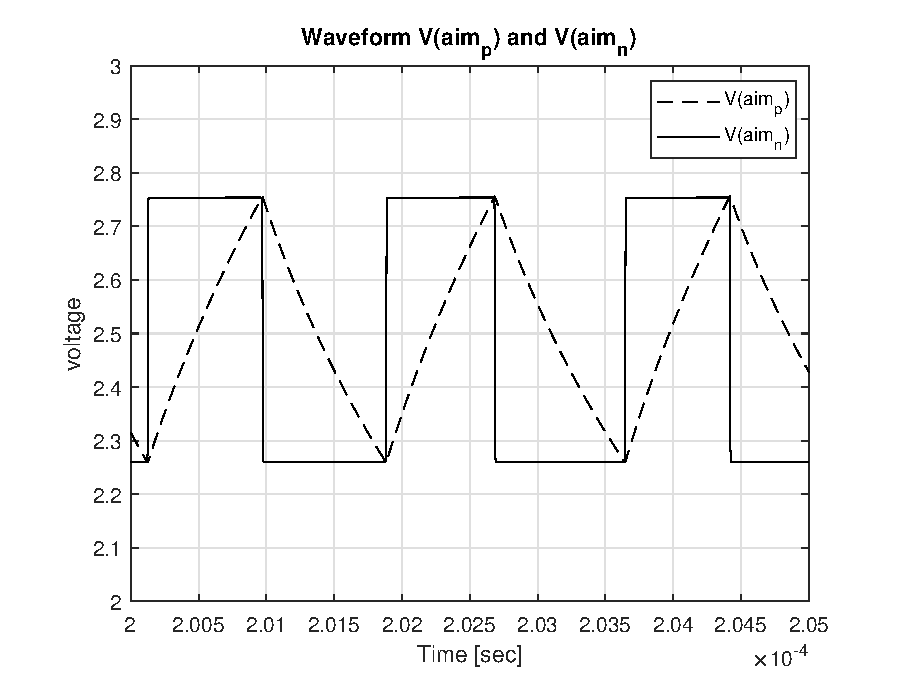
\includegraphics[width=0.8\textwidth]{Analysis/ltspice_aim_hysteresis_window.eps}
	\caption{Hysteresis window on AIM}
	\label{fig:ltspice_aim_hysteresis_window}
\end{figure}
Seen in \autoref{fig:ltspice_aim_hysteresis_window} is the hysteresis window conforming to the theoretical model. The analysis is performed by inputting a DC component of \SI{2.5}{\volt} with zero AC components. This gives a duty cycle of \SI{50}{\percent} and an idle switching frequency of \SI{600}{\kilo\hertz}. It is noted that the variables $V_{\mathrm{th}_{H}}$ and $V_{\mathrm{th}_{L}}$ is seen in the square waveform alternating between \SIrange{2.25}{2.75}{\volt} as mentioned in \Cref{eq:hysteresis_window_synth_a,eq:hysteresis_window_synth_b} and the carrier waveform is seen on the dashed curve. Noted is a slight non-linear curve of the carrier waveform due to the AIM capacitor charge and discharge in each cycle.

\section{Output filter (Calculation and Simulation)}
As a class-D amplifier cannot be classified as a linear time-invariant system, it is difficult to perform a small-signal analysis of the complete circuit with regards to the influence of parasitic elements in the output filter. Therefore, the output filter with various parasitic elements will be investigated using the output stage alone.

\subsection{Analytical approach}
To make nodal analysis more convenient the filter is transformed to single-ended filter type using \Cref{eq:l_ind,eq:c_btl_f,eq:r_btl_f}. 
\begin{figure}[htbp]
	\centering
	\begin{circuitikz}
				\draw (0, -1) coordinate(point1) to[L, l=$L$] ++(2, 0) to[short, -*] ++(2, 0) coordinate(point2) to[C, l_=$C_{f}$, *-*] ++(0, -3) coordinate(point3) to[short, *-] ++(-2, 0) to[short] ++(-2, 0) to[short, -o] ++(-1, 0) coordinate(point4) ;
		\draw (point1) to[short, -o] ++(-1, 0) ;
		\draw (point2) to[short, *-] ++(2, 0) to[R, l_=$R_{f}$] ++(0, -3) to[short, -*] (point3) ;
		\draw (point2) ++(3.2,0) to[open, v=$V_{\mathrm{out}}(s)$] ++(0, -3) (point3) ;
		\draw (point1) ++(-1,0) to[open, v=$V_{\mathrm{in}}(s)$] (point4);
	\end{circuitikz}
	\subcaption{Single-ended output filter}
	\label{fig:analysis_single_ended_lp_filter}
\end{figure}

Applying nodal analysis to \Cref{fig:analysis_single_ended_lp_filter} yields:
\begin{equation} \label{eq:tf_outputfilter_reduction}
	\begin{split}
		H(s) &= \frac{V_{\mathrm{out}}(s)}{V_{\mathrm{in}}(s)} = \frac{ \frac{R_{f}}{1 + s \left(  R_{f}C_{f} \right) }}{sL + \frac{R_{f}}{1 + s \left(  R_{f}C_{f} \right) }} \\
		&= \frac{R_{f}}{R_{f} + sL + s^{2} R_{f}LC_{f}} \\
		&= \frac{1}{1 + s   \frac{L}{R_{f}}  + s^{2} LC_{f}}
	\end{split}
\end{equation}
Finally, from \autoref{eq:tf_outputfilter_reduction} it is seen that the transfer function has no zeros and two poles.

\subsubsection{Inductor parasitic ESR}
\begin{figure}[htbp]
	\centering
	\begin{circuitikz}
				% Single-ended filter version
		\draw (0, -1) coordinate(point1) to[L, l=$L$] ++(2, 0) to[R, l=$R_{ESR}$, -*] ++(2, 0) coordinate(point2) to[C, l_=$C_{f}$, *-*] ++(0, -3) coordinate(point3) to[short, *-] ++(-2, 0) to[short] ++(-2, 0) to[short, -o] ++(-1, 0) coordinate(point4) ;
		\draw (point1) to[short, -o] ++(-1, 0) ;
		\draw (point2) to[short, *-] ++(2, 0) to[R, l_=$R_{f}$] ++(0, -3) to[short, -*] (point3) ;
		\draw (point2) ++(3.2,0) to[open, v=$V_{\mathrm{out}}(s)$] ++(0, -3) (point3) ;
		\draw (point1) ++(-1,0) to[open, v=$V_{\mathrm{in}}(s)$] (point4);
		% Differential filter version
		%		\draw (0, -1) coordinate(point1) to[L, l=$L_{ind}$] ++(2, 0) to[R, l=$R_{ESR}$, -*] ++(2, 0) coordinate(point2) to[C, l_=$C_{BTL}$, *-*] ++(0, -3) coordinate(point3) to[R, l=$R_{ESR}$, *-] ++(-2, 0) to[L, l=$L_{ind}$] ++(-2, 0) to[short, -o] ++(-1, 0) coordinate(point4) ;
		%		\draw (point1) to[short, -o] ++(-1, 0) ;
		%		\draw (point2) to[short, *-] ++(2, 0) to[R, l_=$R_{BTL}$] ++(0, -3) to[short, -*] (point3) ;
		%		\draw (point2) ++(3.2,0) to[open, v=$V_{\mathrm{out}}(s)$] ++(0, -3) (point3) ;
		%		\draw (point1) ++(-1,0) to[open, v=$V_{\mathrm{in}}(s)$] (point4);
	\end{circuitikz}
	\caption{Output filter parasitic elements, addition of series resistance $R_{\mathrm{ESR}}$}
	\label{fig:diagram_output_filter_esr}
\end{figure}
Seen in \autoref{fig:diagram_output_filter_esr} is a diagram of the inserted parasitic series resistance of the output filter inductor. Initial decision of numeric value of inserted parasitic resistance was an choice in desire for sufficient weight of change in behaviour and a sensibility in function. The decision was a resistance value of \SI{300}{\milli\ohm}.

\begin{equation} \label{eq:tf_outputfilter_esr_reduction}
	\begin{split}
		H(s) &= \frac{V_{\mathrm{out}}(s)}{V_{\mathrm{in}}(s)} = \frac{\frac{R_{f}}{1 + sR_{f}C}}{R_{\mathrm{ESR}} + sL_{\mathrm{ind}} + \frac{R_{f}}{1 + sR_{f}C}} \\
		&= \frac{R_{f}}{ \left(  R_{\mathrm{ESR}} + R_{f} \right)  + s(L+R_{f} R_{\mathrm{ESR}}C_{f}) + s^{2} (R_{f}LC_{f})}
	\end{split}
\end{equation}

Looking to \autoref{eq:tf_outputfilter_esr_reduction}, it is seen that the addition of a series resistance to the inductor does not cause addition of a pole or zero which is an indication that the frequency response of the system will not be significantly altered by the series resistance of the inductor.

\subsubsection{Inductor parasitic capacitance}
Decision on a equivalent parallel capacitance of the inductor was made by calculating the resonance frequency of the inductor from earlier impedance analysis and back-calculating for solving for the capacitance using an LC-equation. The resulting value was \SI{120}{\pico\farad}.
\begin{figure}[H]
	\centering
	\begin{circuitikz}
				% Single-ended output filter version
		\draw (0, -1) coordinate(point1) to[L, l_=$L$, *-*] ++(2, 0) coordinate(point2) to[short, *-*] ++(2, 0) coordinate(point3) to[C, l_=$C_{f}$, *-*] ++(0, -3) coordinate(point4) to[short] ++(-2, 0) coordinate(point5) to[short] ++(-2, 0) coordinate(point6) to[short, -o] ++(-1, 0) ;
		\draw (point1) to[short, *-o] ++(-1, 0) ;
		\draw (point1) to[short, *-] ++(0, 1) to[C, l=$C_{s}$] ++(2, 0) coordinate(point7) ;
		\draw (point2) to[short, *-] (point7) ;
		\draw (point3) to[short, *-] ++(2, 0) to[R, l_=$R_{f}$] ++(0, -3) to[short, -*] (point4) ;
		\draw (point3) ++(3.2,0) to[open, v=$V_{\mathrm{out}}(s)$] ++(0,-3) (point4) ;
		\draw (point1) ++(-1,0) to[open, v=$V_{\mathrm{in}}(s)$] ++(0,-3) (point6) ;
		% Differential output filter version
		%		\draw (0, -1) coordinate(point1) to[L, l_=$L_{ind}$, *-*] ++(2, 0) coordinate(point2) to[R, l=$R_{ESR}$, *-*] ++(2, 0) coordinate(point3) to[C, l_=$C_{BTL}$, *-*] ++(0, -3) coordinate(point4) to[R, l=$R_{ESR}$, *-*] ++(-2, 0) coordinate(point5) to[L, l_=$L_{ind}$, *-*] ++(-2, 0) coordinate(point6) to[short, *-o] ++(-1, 0) ;
		%		\draw (point1) to[short, *-o] ++(-1, 0) ;
		%		\draw (point1) to[short, *-] ++(0, 1) to[C, l=$C_{s}$] ++(2, 0) coordinate(point7) ;
		%		\draw (point2) to[short, *-] (point7) ;
		%		\draw (point3) to[short, *-] ++(2, 0) to[R, l_=$R_{BTL}$] ++(0, -3) to[short, -*] (point4) ;
		%		\draw (point5) to[short, *-] ++(0, -1) coordinate(point8) ;
		%		\draw (point6) to[short, *-] ++(0, -1) to[C, l_=$C_{s}$] (point8) ;
		%		\draw (point3) ++(3.2,0) to[open, v=$V_{\mathrm{out}}(s)$] ++(0,-3) (point4) ;
		%		\draw (point1) ++(-1,0) to[open, v=$V_{\mathrm{in}}(s)$] ++(0,-3) (point6) ;
	\end{circuitikz}
	\caption{Output filter parasitic elements, addition of parallel capacitance $C_{s}$}
	\label{fig:diagram_output_filter_c_par}
\end{figure}
Seen in \autoref{fig:diagram_output_filter_c_par} is a diagram of inserted parallel capacitance of inductors.

\begin{equation} \label{eq:tf_outputfilter_parallel_c_reduction}
	\begin{split}
		H(s) &= \frac{V_{\mathrm{out}}(s)}{V_{\mathrm{in}}(s)} = \frac{\frac{R_{f}}{1 + sR_{f}C_{f}}}{\frac{sL}{1+s^{2}LC_{L}} + \frac{R}{1 + sRC}} \\
		&= \frac{R + s^{2} RLC_{L}}{R + sL + s^{2} (RLC_{L} + RLC)} \\
	\end{split}
\end{equation}

From \autoref{eq:tf_outputfilter_parallel_c_reduction} it is seen that a zero is added in the numerator of the transfer function. This indicates a change in the overall response of the system.

\subsubsection{Summary}
In the derived expressions for transfer functions of addition of inductor series resistance and parallel capacitance, it is seen from a control loop stand point that the parallel capacitance makes the most significant change to the frequency response. The location of the zero is presumably rather high in frequency, based on the small capacitor value of \SI{120}{\pico\farad}.

\subsection{Simulation approach}
\begin{figure}[htbp]
	\centering
	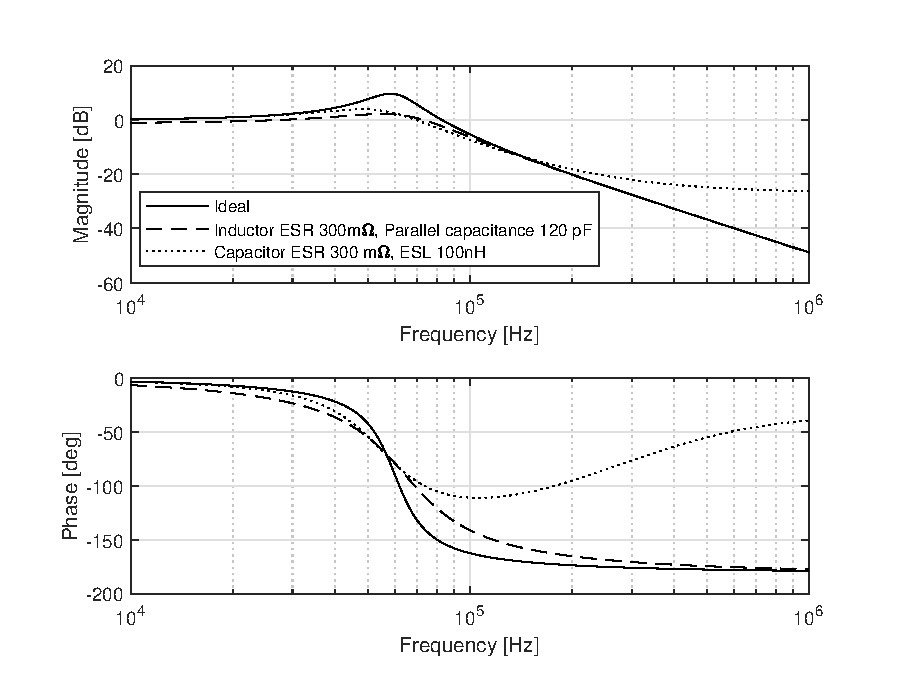
\includegraphics[width=0.8\textwidth]{Analysis/ltspice_output_filter_parasitic.eps}
	\caption{Bode plot of output filter using ideal LC filter, parasitic elements in inductor and parasitic elements in capacitor}
	\label{fig:ltspice_output_filter_l_parasitic}
\end{figure}

Looking at \autoref{fig:ltspice_output_filter_l_parasitic}, different plots are seen of the small-signal output of the output filter. This figure is based of a small-signal analysis from \autoref{fig:ltspice_output_filter_smallsignal}. First the ideal filter is plotted and contains a relatively prominent peak around the cut-off frequency. This is by design, as the Q factor is relatively high. This resonance peak was decided to compensate for some switching losses in the power stage. It is noted that as parasitic elements are added in the inductor and capacitor, this resonance peak is lowered and will presumably cause further switching losses in the output stage. In the magnitude plot it can be seen that overall, the parasitic elements in the capacitor seem to make a larger change to the frequency response in the high-frequency range.

\section{Initial tests (Hardware)}
A preliminary analysis was attempted to be made on the hardware. Unfortunately, there were stability issues with the setup. Differential voltage measurements made across the load revealed through-put of the amplified input signal, with a high-frequent oscillation superimposed. On rough estimates, the high-frequent oscillation signal appeared to be in the vicinity of the resonance frequency of the output filter. Shortly thereafter during testing, the lower half-bridge short-circuited, and reparation of the hardware was necessary. After repairs were completed on the amplifier circuit and tested to be functional, next will be some hardware analysis on the circuitry.

\section{Control loop (Hardware)}
Regulator characteristics for amplifier circuitry are determined by its converter loop transfer function. This transfer function can be illustrated by a Bode plot. This representation of magnitude and phase over a frequency spectrum gives insight into the speed of the regulation loop and the general stability of the system. To acquire the Bode plot data measurements need to be made on the circuit. This will be explained in the following sections.

\subsection{Measurement setup}
A measurement setup is implemented using a Bode 100 Vector Network Analyzer \cite{bode100_manual}. To determine the control loop parameters of an active circuit, a wideband injection transformer is required. Using the recommended typical measurement setup from \autoref{fig:injection_transformer_setup}, the following measurement setup is implemented:

\begin{figure}[htbp]
	\centering
	\adjustbox{max width=\textwidth}{%
	

\tikzset{every picture/.style={line width=0.75pt}} %set default line width to 0.75pt        

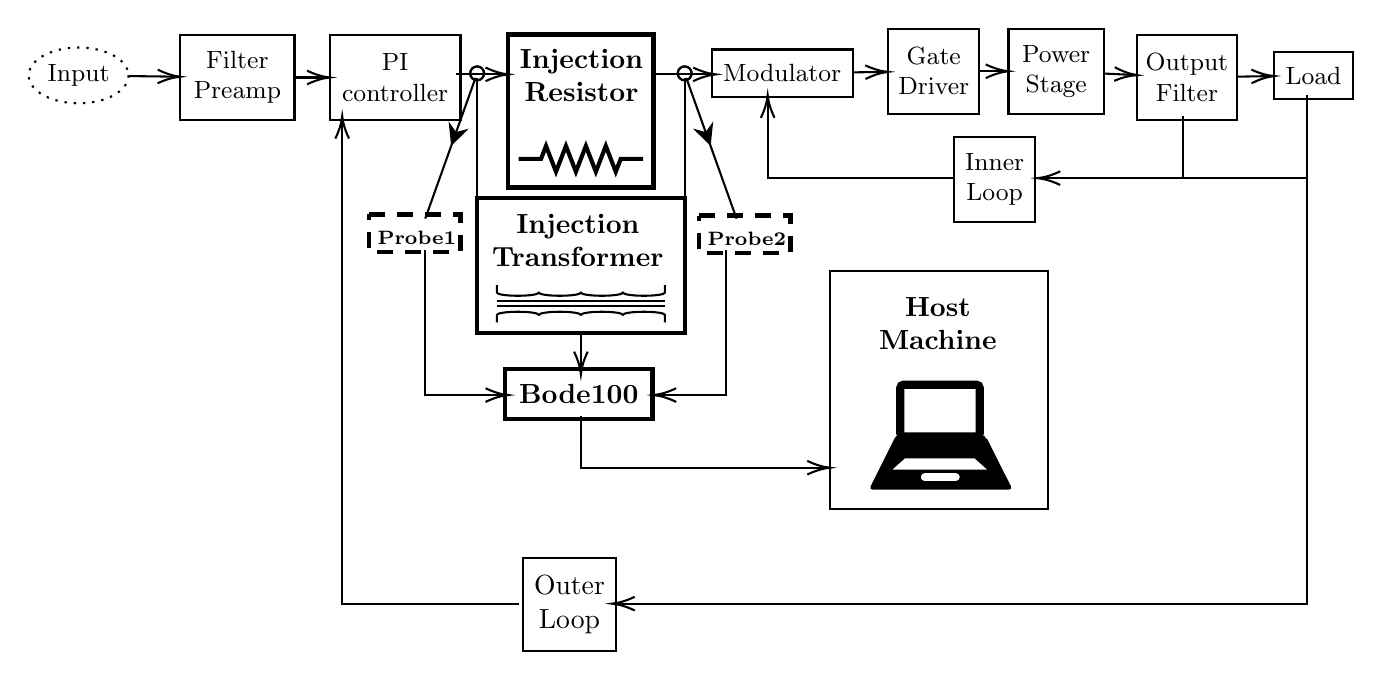
\begin{tikzpicture}[x=0.75pt,y=0.75pt,yscale=-1,xscale=1]
	%uncomment if require: \path (0,319); %set diagram left start at 0, and has height of 319
	
	%Straight Lines [id:da15735186867115303] 
	\draw    (380,114.51) ;
	%Shape: Resistor [id:dp9057667935403209] 
	\draw  [line width=1.5]  (240,70.7) -- (250.8,70.7) -- (253.2,64.51) -- (258,76.89) -- (262.8,64.51) -- (267.6,76.89) -- (272.4,64.51) -- (277.2,76.89) -- (282,64.51) -- (286.8,76.89) -- (289.2,70.7) -- (300,70.7) ;
	%Shape: Rectangle [id:dp3413763907901186] 
	\draw  [line width=1.5]  (235,10.8) -- (305,10.8) -- (305,84.51) -- (235,84.51) -- cycle ;
	
	%Shape: Rectangle [id:dp11748765664080651] 
	\draw  [line width=1.5]  (220,89.51) -- (320,89.51) -- (320,154.51) -- (220,154.51) -- cycle ;
	%Shape: Inductor [id:dp2215516061269578] 
	\draw   (310.48,131.51) -- (310.48,135.14) .. controls (310.48,135.98) and (305.94,136.66) .. (300.36,136.66) .. controls (294.77,136.66) and (290.24,135.98) .. (290.24,135.14) .. controls (290.24,135.98) and (285.7,136.66) .. (280.12,136.66) .. controls (274.53,136.66) and (270,135.98) .. (270,135.14) .. controls (270,135.98) and (265.47,136.66) .. (259.88,136.66) .. controls (254.3,136.66) and (249.76,135.98) .. (249.76,135.14) .. controls (249.76,135.98) and (245.23,136.66) .. (239.64,136.66) .. controls (234.06,136.66) and (229.52,135.98) .. (229.52,135.14) -- (229.52,131.51) ;
	%Shape: Inductor [id:dp6400099710814144] 
	\draw   (229.52,149.51) -- (229.52,145.88) .. controls (229.52,145.05) and (234.06,144.37) .. (239.64,144.37) .. controls (245.23,144.37) and (249.76,145.05) .. (249.76,145.88) .. controls (249.76,145.05) and (254.3,144.37) .. (259.88,144.37) .. controls (265.47,144.37) and (270,145.05) .. (270,145.88) .. controls (270,145.05) and (274.53,144.37) .. (280.12,144.37) .. controls (285.7,144.37) and (290.24,145.05) .. (290.24,145.88) .. controls (290.24,145.05) and (294.77,144.37) .. (300.36,144.37) .. controls (305.94,144.37) and (310.48,145.05) .. (310.48,145.88) -- (310.48,149.51) ;
	%Straight Lines [id:da2673964347130813] 
	\draw    (310.48,139.23) -- (229.52,139.23) ;
	%Straight Lines [id:da09279762971391459] 
	\draw    (310.48,141.8) -- (229.52,141.8) ;
	
	
	%Straight Lines [id:da2761001544350641] 
	\draw    (220,89.51) -- (220,31.86) ;
	\draw [shift={(220,29.51)}, rotate = 270] [color={rgb, 255:red, 0; green, 0; blue, 0 }  ][line width=0.75]      (0, 0) circle [x radius= 3.35, y radius= 3.35]   ;
	%Straight Lines [id:da3809757606569024] 
	\draw    (320,89.51) -- (320,31.86) ;
	\draw [shift={(320,29.51)}, rotate = 270] [color={rgb, 255:red, 0; green, 0; blue, 0 }  ][line width=0.75]      (0, 0) circle [x radius= 3.35, y radius= 3.35]   ;
	%Straight Lines [id:da5383504403874997] 
	\draw    (270,154.51) -- (270,172.51) ;
	\draw [shift={(270,174.51)}, rotate = 270] [color={rgb, 255:red, 0; green, 0; blue, 0 }  ][line width=0.75]    (10.93,-3.29) .. controls (6.95,-1.4) and (3.31,-0.3) .. (0,0) .. controls (3.31,0.3) and (6.95,1.4) .. (10.93,3.29)   ;
	%Straight Lines [id:da299918873882153] 
	\draw    (195,99.51) -- (219.21,31.73) ;
	\draw [shift={(220,29.51)}, rotate = 289.65] [color={rgb, 255:red, 0; green, 0; blue, 0 }  ][line width=0.75]      (0, 0) circle [x radius= 3.35, y radius= 3.35]   ;
	\draw [shift={(207.5,64.51)}, rotate = 289.65] [fill={rgb, 255:red, 0; green, 0; blue, 0 }  ][line width=0.08]  [draw opacity=0] (10.72,-5.15) -- (0,0) -- (10.72,5.15) -- (7.12,0) -- cycle    ;
	%Straight Lines [id:da15762166605604144] 
	\draw    (345,99.51) -- (320.79,31.73) ;
	\draw [shift={(320,29.51)}, rotate = 250.35] [color={rgb, 255:red, 0; green, 0; blue, 0 }  ][line width=0.75]      (0, 0) circle [x radius= 3.35, y radius= 3.35]   ;
	\draw [shift={(332.5,64.51)}, rotate = 250.35] [fill={rgb, 255:red, 0; green, 0; blue, 0 }  ][line width=0.08]  [draw opacity=0] (10.72,-5.15) -- (0,0) -- (10.72,5.15) -- (7.12,0) -- cycle    ;
	%Straight Lines [id:da21183603730332523] 
	\draw    (233,184.51) -- (195,184.51) -- (195,114.51) ;
	\draw [shift={(235,184.51)}, rotate = 180] [color={rgb, 255:red, 0; green, 0; blue, 0 }  ][line width=0.75]    (10.93,-3.29) .. controls (6.95,-1.4) and (3.31,-0.3) .. (0,0) .. controls (3.31,0.3) and (6.95,1.4) .. (10.93,3.29)   ;
	%Straight Lines [id:da9973840816661179] 
	\draw    (307,184.51) -- (340,184.51) -- (340,114.51) ;
	\draw [shift={(305,184.51)}, rotate = 0] [color={rgb, 255:red, 0; green, 0; blue, 0 }  ][line width=0.75]    (10.93,-3.29) .. controls (6.95,-1.4) and (3.31,-0.3) .. (0,0) .. controls (3.31,0.3) and (6.95,1.4) .. (10.93,3.29)   ;
	%Straight Lines [id:da02531886687147078] 
	\draw    (560,50) -- (560,80) -- (492,80) ;
	\draw [shift={(490,80)}, rotate = 360] [color={rgb, 255:red, 0; green, 0; blue, 0 }  ][line width=0.75]    (10.93,-3.29) .. controls (6.95,-1.4) and (3.31,-0.3) .. (0,0) .. controls (3.31,0.3) and (6.95,1.4) .. (10.93,3.29)   ;
	%Straight Lines [id:da9679903044516098] 
	\draw    (620,80) -- (490,80) ;
	%Straight Lines [id:da8177057617014005] 
	\draw    (450,80) -- (360,80) -- (360,42) ;
	\draw [shift={(360,40)}, rotate = 450] [color={rgb, 255:red, 0; green, 0; blue, 0 }  ][line width=0.75]    (10.93,-3.29) .. controls (6.95,-1.4) and (3.31,-0.3) .. (0,0) .. controls (3.31,0.3) and (6.95,1.4) .. (10.93,3.29)   ;
	%Straight Lines [id:da44249742206669795] 
	\draw    (240,285) -- (155,285) -- (155,52) ;
	\draw [shift={(155,50)}, rotate = 450] [color={rgb, 255:red, 0; green, 0; blue, 0 }  ][line width=0.75]    (10.93,-3.29) .. controls (6.95,-1.4) and (3.31,-0.3) .. (0,0) .. controls (3.31,0.3) and (6.95,1.4) .. (10.93,3.29)   ;
	%Straight Lines [id:da434984126138388] 
	\draw    (620,40) -- (620,285) -- (287,285) ;
	\draw [shift={(285,285)}, rotate = 360] [color={rgb, 255:red, 0; green, 0; blue, 0 }  ][line width=0.75]    (10.93,-3.29) .. controls (6.95,-1.4) and (3.31,-0.3) .. (0,0) .. controls (3.31,0.3) and (6.95,1.4) .. (10.93,3.29)   ;
	%Rounded Rect [id:dp5356236767557228] 
	\draw  [line width=3]  (423.89,181.22) .. controls (423.89,180.28) and (424.65,179.51) .. (425.6,179.51) -- (460.44,179.51) .. controls (461.38,179.51) and (462.14,180.28) .. (462.14,181.22) -- (462.14,202.81) .. controls (462.14,203.75) and (461.38,204.51) .. (460.44,204.51) -- (425.6,204.51) .. controls (424.65,204.51) and (423.89,203.75) .. (423.89,202.81) -- cycle ;
	%Shape: Path Data [id:dp8744529124252245] 
	\draw  [fill={rgb, 255:red, 0; green, 0; blue, 0 }  ,fill opacity=1 ] (423.08,204.51) -- (463.72,204.51) .. controls (464.24,204.51) and (464.45,204.93) .. (464.19,205.45) .. controls (464.69,205.45) and (465.3,205.86) .. (465.55,206.35) -- (476.69,228.61) .. controls (476.94,229.11) and (476.74,229.51) .. (476.24,229.51) -- (410.58,229.51) .. controls (410.06,229.51) and (409.85,229.09) .. (410.11,228.58) -- (421.68,205.45) .. controls (421.93,204.93) and (422.56,204.51) .. (423.08,204.51) -- cycle ;
	%Shape: Path Data [id:dp07874170081554621] 
	\draw  [fill={rgb, 255:red, 255; green, 255; blue, 255 }  ,fill opacity=1 ] (418.64,220.94) -- (425.9,214.51) -- (459.89,214.51) -- (467.14,220.94) -- (418.64,220.94) -- cycle ;
	%Rounded Rect [id:dp13746892324163995] 
	\draw  [fill={rgb, 255:red, 255; green, 255; blue, 255 }  ,fill opacity=1 ] (433.14,224.01) .. controls (433.14,222.63) and (434.26,221.51) .. (435.64,221.51) -- (450.64,221.51) .. controls (452.02,221.51) and (453.14,222.63) .. (453.14,224.01) -- (453.14,224.01) .. controls (453.14,225.39) and (452.02,226.51) .. (450.64,226.51) -- (435.64,226.51) .. controls (434.26,226.51) and (433.14,225.39) .. (433.14,224.01) -- cycle ;
	
	%Shape: Rectangle [id:dp8051019294222979] 
	\draw   (390,124.51) -- (495,124.51) -- (495,239.51) -- (390,239.51) -- cycle ;
	
	%Straight Lines [id:da7928450406272949] 
	\draw    (270,194.51) -- (270,219.51) -- (388,219.51) ;
	\draw [shift={(390,219.51)}, rotate = 180] [color={rgb, 255:red, 0; green, 0; blue, 0 }  ][line width=0.75]    (10.93,-3.29) .. controls (6.95,-1.4) and (3.31,-0.3) .. (0,0) .. controls (3.31,0.3) and (6.95,1.4) .. (10.93,3.29)   ;
	%Straight Lines [id:da3870728561566599] 
	\draw    (210,30) -- (233,30) ;
	\draw [shift={(235,30)}, rotate = 180] [color={rgb, 255:red, 0; green, 0; blue, 0 }  ][line width=0.75]    (10.93,-3.29) .. controls (6.95,-1.4) and (3.31,-0.3) .. (0,0) .. controls (3.31,0.3) and (6.95,1.4) .. (10.93,3.29)   ;
	%Straight Lines [id:da028020813655613486] 
	\draw    (305,30) -- (333,30) ;
	\draw [shift={(335,30)}, rotate = 180] [color={rgb, 255:red, 0; green, 0; blue, 0 }  ][line width=0.75]    (10.93,-3.29) .. controls (6.95,-1.4) and (3.31,-0.3) .. (0,0) .. controls (3.31,0.3) and (6.95,1.4) .. (10.93,3.29)   ;
	
	% Text Node
	\draw    (333,18) -- (401,18) -- (401,41) -- (333,41) -- cycle  ;
	\draw (367,29.5) node  [font=\small] [align=left] {\begin{minipage}[lt]{43.538224pt}\setlength\topsep{0pt}
			\begin{center}
				Modulator
			\end{center}
			
	\end{minipage}};
	% Text Node
	\draw    (77,11) -- (132,11) -- (132,52) -- (77,52) -- cycle  ;
	\draw (104.5,31.5) node  [font=\small] [align=left] {\begin{minipage}[lt]{34.862172pt}\setlength\topsep{0pt}
			\begin{center}
				Filter\\Preamp
			\end{center}
			
	\end{minipage}};
	% Text Node
	\draw  [dash pattern={on 0.84pt off 2.51pt}]  (28, 30.5) circle [x radius= 24.04, y radius= 13.44]   ;
	\draw (28,30.5) node  [font=\small] [align=left] {\begin{minipage}[lt]{23.138224pt}\setlength\topsep{0pt}
			\begin{center}
				Input
			\end{center}
			
	\end{minipage}};
	% Text Node
	\draw    (418,8) -- (462,8) -- (462,49) -- (418,49) -- cycle  ;
	\draw (440,28.5) node  [font=\small] [align=left] {\begin{minipage}[lt]{27.193948000000002pt}\setlength\topsep{0pt}
			\begin{center}
				Gate\\Driver
			\end{center}
			
	\end{minipage}};
	% Text Node
	\draw    (476,8) -- (522,8) -- (522,49) -- (476,49) -- cycle  ;
	\draw (499,28.5) node  [font=\small] [align=left] {\begin{minipage}[lt]{28.736052pt}\setlength\topsep{0pt}
			\begin{center}
				Power\\Stage
			\end{center}
			
	\end{minipage}};
	% Text Node
	\draw    (538,11) -- (586,11) -- (586,52) -- (538,52) -- cycle  ;
	\draw (562,31.5) node  [font=\small] [align=left] {\begin{minipage}[lt]{30.272172pt}\setlength\topsep{0pt}
			\begin{center}
				Output\\Filter
			\end{center}
			
	\end{minipage}};
	% Text Node
	\draw  [line width=0.75]   (604,19) -- (642,19) -- (642,42) -- (604,42) -- cycle  ;
	\draw (623,30.5) node  [font=\small] [align=left] {\begin{minipage}[lt]{23.138224pt}\setlength\topsep{0pt}
			\begin{center}
				Load
			\end{center}
			
	\end{minipage}};
	% Text Node
	\draw    (449.86,60) -- (488.86,60) -- (488.86,101) -- (449.86,101) -- cycle  ;
	\draw (469.36,80.5) node  [font=\small] [align=left] {\begin{minipage}[lt]{23.642172pt}\setlength\topsep{0pt}
			\begin{center}
				Inner\\Loop
			\end{center}
			
	\end{minipage}};
	% Text Node
	\draw    (242,263) -- (287,263) -- (287,308) -- (242,308) -- cycle  ;
	\draw (264.5,285.5) node   [align=left] {\begin{minipage}[lt]{28.232172pt}\setlength\topsep{0pt}
			\begin{center}
				Outer\\Loop
			\end{center}
			
	\end{minipage}};
	% Text Node
	\draw    (149,11) -- (212,11) -- (212,52) -- (149,52) -- cycle  ;
	\draw (180.5,31.5) node  [font=\small] [align=left] {\begin{minipage}[lt]{40.472172pt}\setlength\topsep{0pt}
			\begin{center}
				PI\\controller
			\end{center}
			
	\end{minipage}};
	% Text Node
	\draw  [line width=1.5]   (233.5,172.01) -- (304.5,172.01) -- (304.5,196.01) -- (233.5,196.01) -- cycle  ;
	\draw (269,184.01) node   [align=left] {\begin{minipage}[lt]{45.244276000000006pt}\setlength\topsep{0pt}
			\begin{center}
				\textbf{Bode100}
			\end{center}
			
	\end{minipage}};
	% Text Node
	\draw  [dash pattern={on 5.63pt off 4.5pt}][line width=1.5]   (168,97.51) -- (212,97.51) -- (212,115.51) -- (168,115.51) -- cycle  ;
	\draw (190,106.51) node  [font=\scriptsize] [align=left] {\begin{minipage}[lt]{26.920724000000003pt}\setlength\topsep{0pt}
			\begin{center}
				\textbf{Probe1}
			\end{center}
			
	\end{minipage}};
	% Text Node
	\draw  [dash pattern={on 5.63pt off 4.5pt}][line width=1.5]   (327,98.01) -- (371,98.01) -- (371,116.01) -- (327,116.01) -- cycle  ;
	\draw (349,107.01) node  [font=\scriptsize] [align=left] {\begin{minipage}[lt]{26.920724000000003pt}\setlength\topsep{0pt}
			\begin{center}
				\textbf{Probe2}
			\end{center}
			
	\end{minipage}};
	% Text Node
	\draw (270.29,30.5) node   [align=left] {\begin{minipage}[lt]{44.66144800000001pt}\setlength\topsep{0pt}
			\begin{center}
				\textbf{Injection}\\\textbf{Resistor}
			\end{center}
			
	\end{minipage}};
	% Text Node
	\draw (268.53,110.01) node   [align=left] {\begin{minipage}[lt]{62.244276000000006pt}\setlength\topsep{0pt}
			\begin{center}
				\textbf{Injection}\\\textbf{Transformer}
			\end{center}
			
	\end{minipage}};
	% Text Node
	\draw (442,150.01) node   [align=left] {\begin{minipage}[lt]{43.532172pt}\setlength\topsep{0pt}
			\begin{center}
				\textbf{Host}\\\textbf{Machine}
			\end{center}
			
	\end{minipage}};
	% Connection
	\draw    (462,28.5) -- (474,28.5) ;
	\draw [shift={(476,28.5)}, rotate = 180] [color={rgb, 255:red, 0; green, 0; blue, 0 }  ][line width=0.75]    (10.93,-3.29) .. controls (6.95,-1.4) and (3.31,-0.3) .. (0,0) .. controls (3.31,0.3) and (6.95,1.4) .. (10.93,3.29)   ;
	% Connection
	\draw    (522,29.6) -- (536,30.26) ;
	\draw [shift={(538,30.36)}, rotate = 182.73] [color={rgb, 255:red, 0; green, 0; blue, 0 }  ][line width=0.75]    (10.93,-3.29) .. controls (6.95,-1.4) and (3.31,-0.3) .. (0,0) .. controls (3.31,0.3) and (6.95,1.4) .. (10.93,3.29)   ;
	% Connection
	\draw    (586,31.11) -- (602,30.84) ;
	\draw [shift={(604,30.81)}, rotate = 539.06] [color={rgb, 255:red, 0; green, 0; blue, 0 }  ][line width=0.75]    (10.93,-3.29) .. controls (6.95,-1.4) and (3.31,-0.3) .. (0,0) .. controls (3.31,0.3) and (6.95,1.4) .. (10.93,3.29)   ;
	% Connection
	\draw    (52.04,30.81) -- (75,31.11) ;
	\draw [shift={(77,31.14)}, rotate = 180.75] [color={rgb, 255:red, 0; green, 0; blue, 0 }  ][line width=0.75]    (10.93,-3.29) .. controls (6.95,-1.4) and (3.31,-0.3) .. (0,0) .. controls (3.31,0.3) and (6.95,1.4) .. (10.93,3.29)   ;
	% Connection
	\draw    (401,29.03) -- (416,28.83) ;
	\draw [shift={(418,28.8)}, rotate = 539.22] [color={rgb, 255:red, 0; green, 0; blue, 0 }  ][line width=0.75]    (10.93,-3.29) .. controls (6.95,-1.4) and (3.31,-0.3) .. (0,0) .. controls (3.31,0.3) and (6.95,1.4) .. (10.93,3.29)   ;
	% Connection
	\draw    (132,31.5) -- (147,31.5) ;
	\draw [shift={(149,31.5)}, rotate = 180] [color={rgb, 255:red, 0; green, 0; blue, 0 }  ][line width=0.75]    (10.93,-3.29) .. controls (6.95,-1.4) and (3.31,-0.3) .. (0,0) .. controls (3.31,0.3) and (6.95,1.4) .. (10.93,3.29)   ;
	
\end{tikzpicture}

	}%
	\caption{Block diagram of measurement setup for transformer injection measurement of control loop}
	\label{fig:block_diagram_transformer_injection}
\end{figure}

Seen in \autoref{fig:block_diagram_transformer_injection} is an overall block diagram of the measurement setup. The Injection Transformer B-WIT 100 transformer \cite{injection_transformer_manual} is used with an injection resistor of \SI{10}{\ohm} inserted in the feed-forward loop between the PI controller and the modulator subcircuits. Typically the injection transformer is inserted across the injection resistor in the feedback loop as per the manual diagram, but to secure the equipment from common-mode voltages, it was decided to break the loop in the low voltage circuitry between the PI controller and the modulator. A breakout board was made using a copper-clad circular perf board, connectors, a resistor and cables. In this project, any reactive characteristics from the speaker will be disregarded. In the practical measurement setup, it will be replaced by a resistive element. Choosing packages for the introduced parasitic elements was based on availability. For the inductor series resistance, three \SI{0.1}{\ohm} was connected in series. For the inductor parallel capacitance, the chosen package was a ceramic 0603 \SI{120}{\pico\farad} capacitor.

\begin{figure}[htbp]
	\centering
	\tcbox{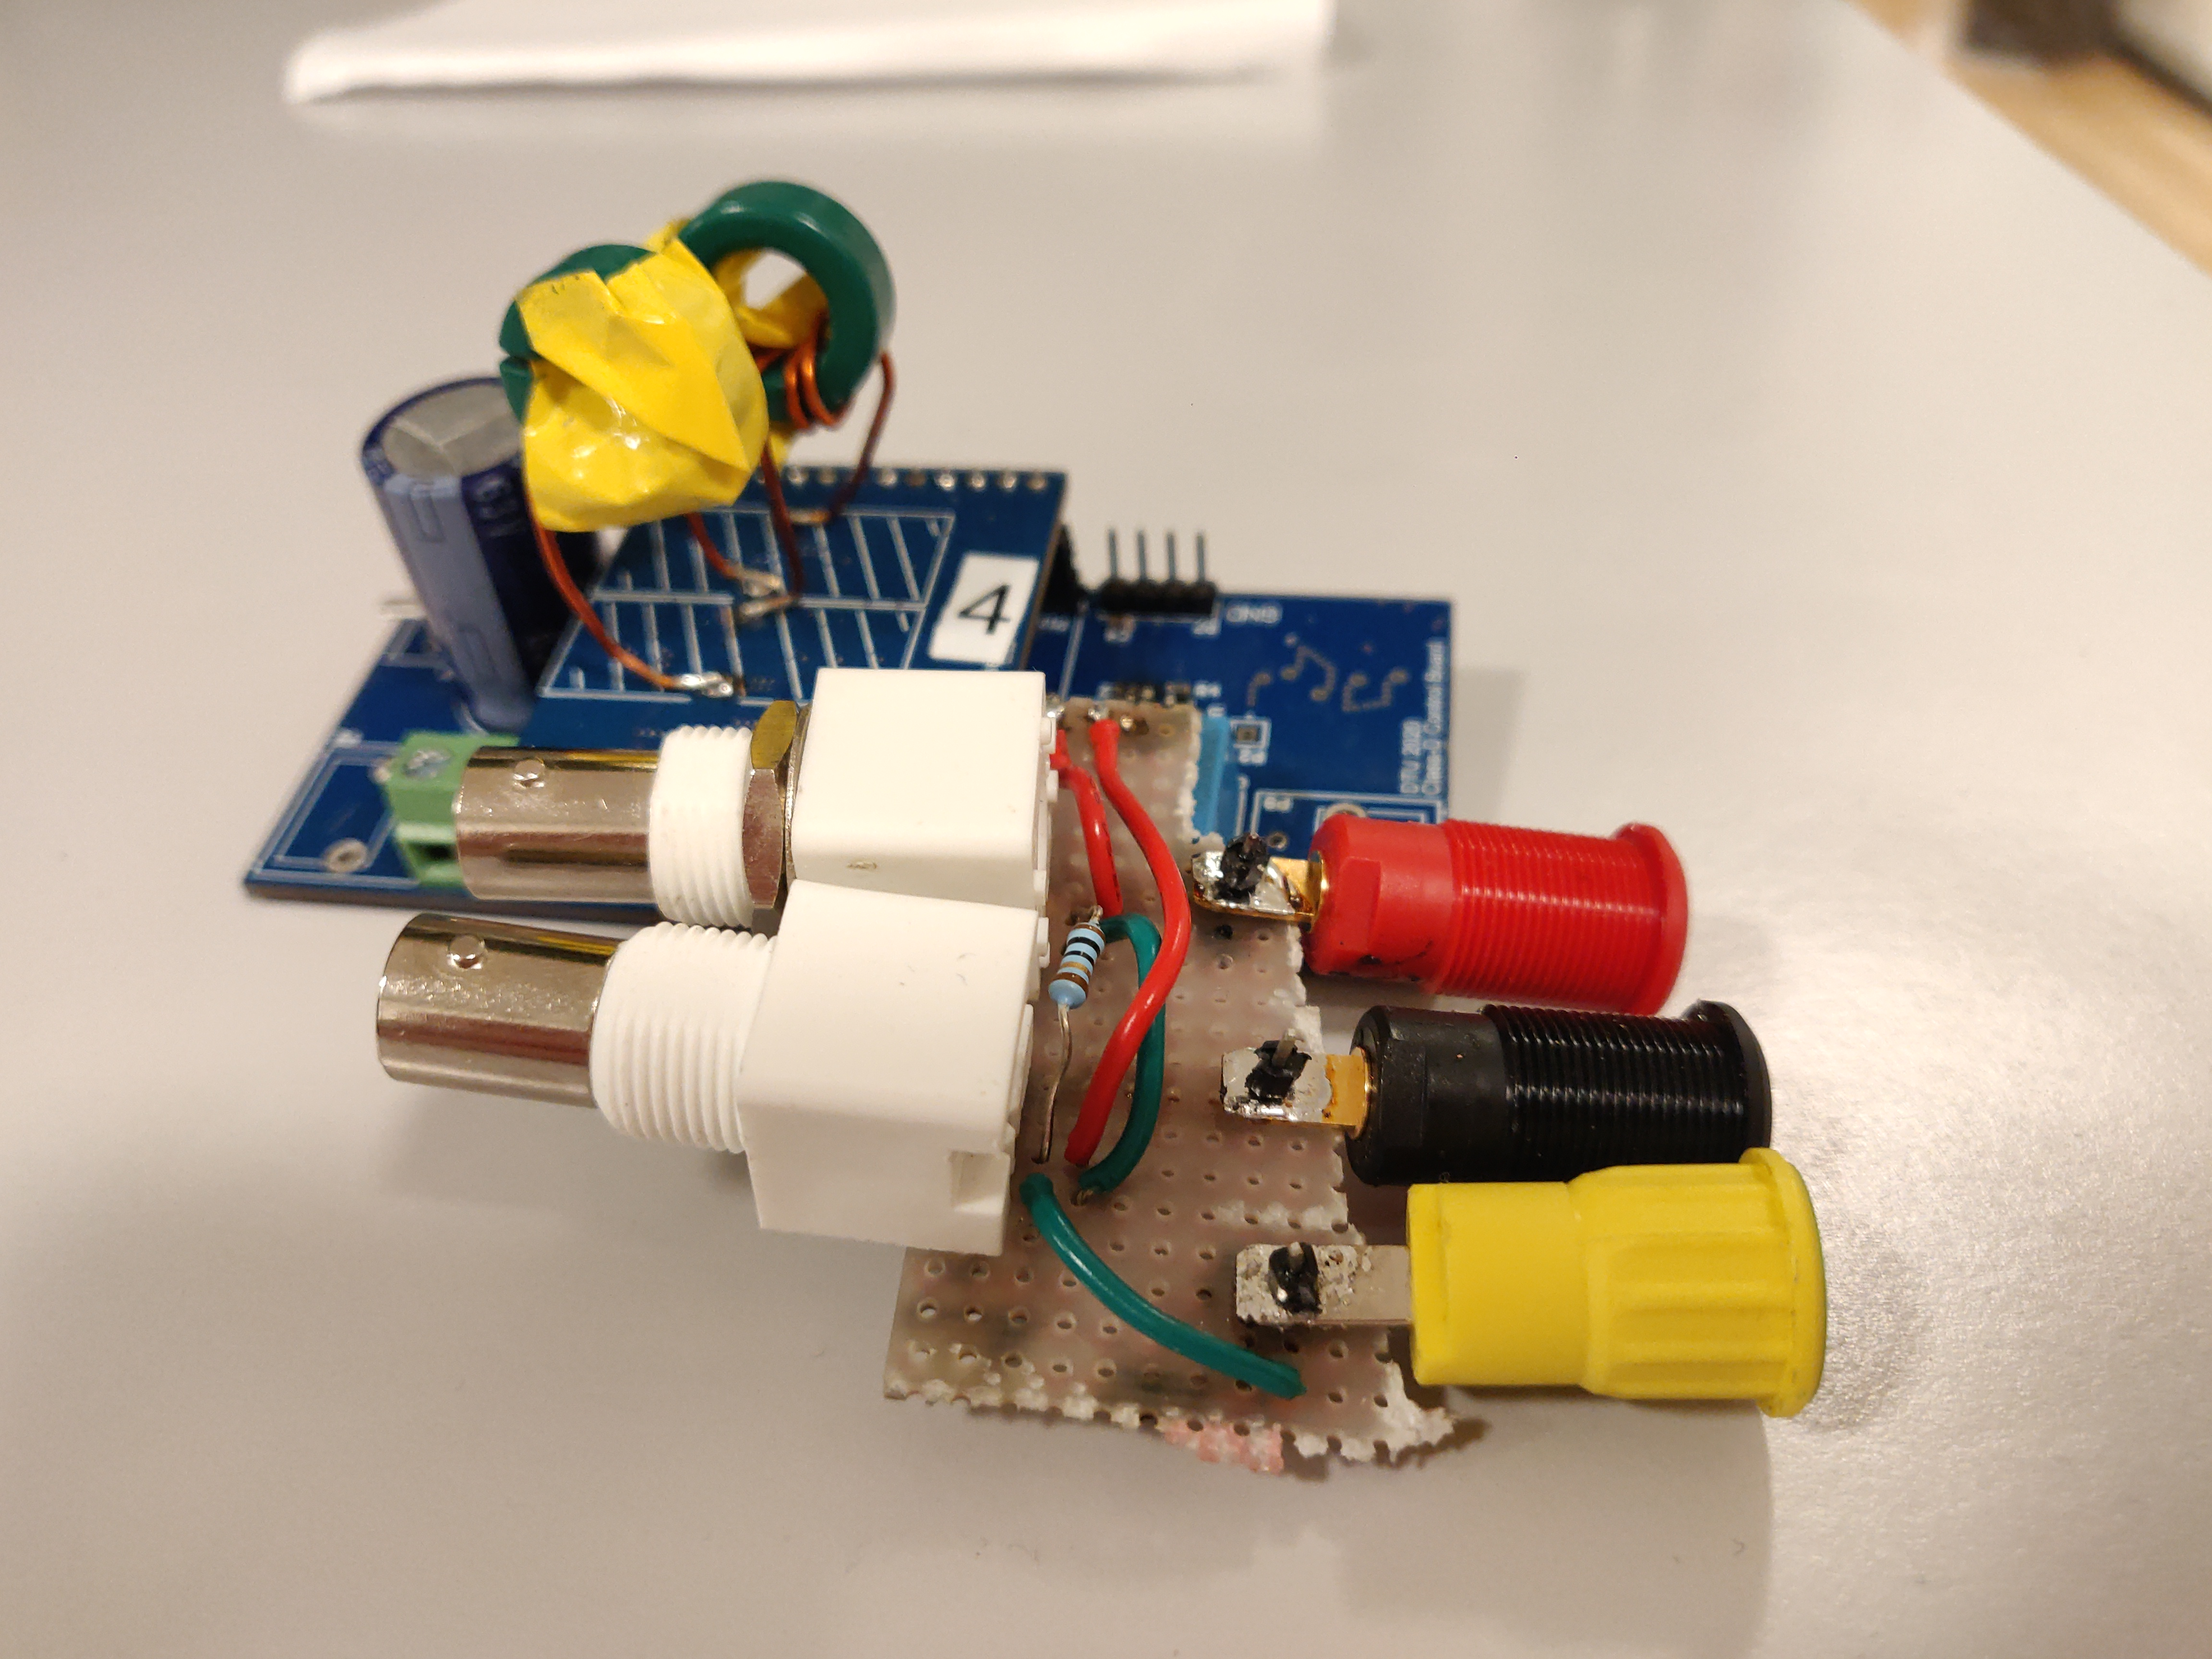
\includegraphics[width=0.8\textwidth, trim=0 0 20cm 10cm, clip]{Analysis/bode100_breakout_board.jpg}}
	\caption{Breakout board for transformer injection measurement setup}
	\label{fig:bode100_breakout_board}
\end{figure}
The breakout board can be seen in \autoref{fig:bode100_breakout_board} mounted on the IO PCB of the amplifier. The two BNC connectors are for Probe 1 and Probe 2 of the Bode 100 Network Vector Analyzer. The red and black \SI{4}{\milli\meter} lab connectors are for the injection transformer. Finally, the green/yellow \SI{4}{\milli\meter} lab connector is for a ground reference on the analyzer probes.



\subsection{Outer loop open, inner loop closed}
\begin{figure}[H]
	\centering
	

\tikzset{every picture/.style={line width=0.75pt}} %set default line width to 0.75pt        

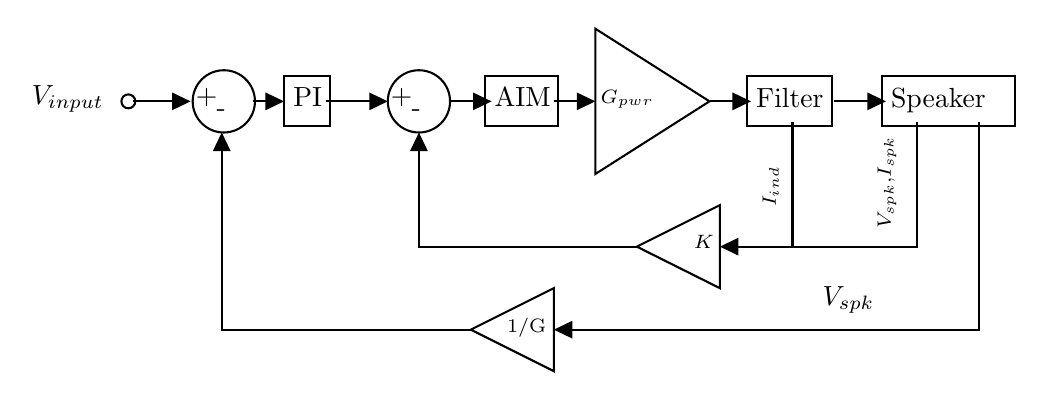
\begin{tikzpicture}[x=0.75pt,y=0.75pt,yscale=-1,xscale=1]
%uncomment if require: \path (0,888); %set diagram left start at 0, and has height of 888

%Shape: Circle [id:dp8093593830625807] 
\draw   (185,45) .. controls (185,36.72) and (191.72,30) .. (200,30) .. controls (208.28,30) and (215,36.72) .. (215,45) .. controls (215,53.28) and (208.28,60) .. (200,60) .. controls (191.72,60) and (185,53.28) .. (185,45) -- cycle ;

%Shape: Triangle [id:dp44581617276213614] 
\draw   (340,45) -- (285,80) -- (285,10) -- cycle ;
%Shape: Triangle [id:dp09631385215595478] 
\draw   (305,115) -- (345,95) -- (345,135) -- cycle ;
%Shape: Triangle [id:dp2526326760327633] 
\draw   (225,155) -- (265,135) -- (265,175) -- cycle ;
%Straight Lines [id:da22947722616995136] 
\draw    (120,45) -- (132,45) ;
\draw [shift={(135,45)}, rotate = 180] [fill={rgb, 255:red, 0; green, 0; blue, 0 }  ][line width=0.08]  [draw opacity=0] (8.93,-4.29) -- (0,0) -- (8.93,4.29) -- cycle    ;
%Straight Lines [id:da9820289371822846] 
\draw    (155,45) -- (182,45) ;
\draw [shift={(185,45)}, rotate = 180] [fill={rgb, 255:red, 0; green, 0; blue, 0 }  ][line width=0.08]  [draw opacity=0] (8.93,-4.29) -- (0,0) -- (8.93,4.29) -- cycle    ;
%Straight Lines [id:da1710685770143594] 
\draw    (215,45) -- (232,45) ;
\draw [shift={(235,45)}, rotate = 180] [fill={rgb, 255:red, 0; green, 0; blue, 0 }  ][line width=0.08]  [draw opacity=0] (8.93,-4.29) -- (0,0) -- (8.93,4.29) -- cycle    ;
%Straight Lines [id:da8296107958731653] 
\draw    (265,45) -- (282,45) ;
\draw [shift={(285,45)}, rotate = 180] [fill={rgb, 255:red, 0; green, 0; blue, 0 }  ][line width=0.08]  [draw opacity=0] (8.93,-4.29) -- (0,0) -- (8.93,4.29) -- cycle    ;
%Straight Lines [id:da7610584415564716] 
\draw    (340,45) -- (357,45) ;
\draw [shift={(360,45)}, rotate = 180] [fill={rgb, 255:red, 0; green, 0; blue, 0 }  ][line width=0.08]  [draw opacity=0] (8.93,-4.29) -- (0,0) -- (8.93,4.29) -- cycle    ;
%Straight Lines [id:da0317255178938578] 
\draw    (400,45) -- (422,45) ;
\draw [shift={(425,45)}, rotate = 180] [fill={rgb, 255:red, 0; green, 0; blue, 0 }  ][line width=0.08]  [draw opacity=0] (8.93,-4.29) -- (0,0) -- (8.93,4.29) -- cycle    ;
%Straight Lines [id:da47831470158494027] 
\draw    (380,55) -- (380,115) -- (348,115) ;
\draw [shift={(345,115)}, rotate = 360] [fill={rgb, 255:red, 0; green, 0; blue, 0 }  ][line width=0.08]  [draw opacity=0] (8.93,-4.29) -- (0,0) -- (8.93,4.29) -- cycle    ;
%Straight Lines [id:da7707722284057568] 
\draw    (440,55) -- (440,115) -- (380,115) ;
%Straight Lines [id:da885640579095621] 
\draw    (470,55) -- (470,155) -- (268,155) ;
\draw [shift={(265,155)}, rotate = 360] [fill={rgb, 255:red, 0; green, 0; blue, 0 }  ][line width=0.08]  [draw opacity=0] (8.93,-4.29) -- (0,0) -- (8.93,4.29) -- cycle    ;
%Straight Lines [id:da06407371574232901] 
\draw    (305,115) -- (200,115) -- (200,63) ;
\draw [shift={(200,60)}, rotate = 450] [fill={rgb, 255:red, 0; green, 0; blue, 0 }  ][line width=0.08]  [draw opacity=0] (8.93,-4.29) -- (0,0) -- (8.93,4.29) -- cycle    ;
%Straight Lines [id:da6120868731529776] 
\draw    (225,155) -- (105,155) -- (105,63) ;
\draw [shift={(105,60)}, rotate = 450] [fill={rgb, 255:red, 0; green, 0; blue, 0 }  ][line width=0.08]  [draw opacity=0] (8.93,-4.29) -- (0,0) -- (8.93,4.29) -- cycle    ;
%Straight Lines [id:da2237355312459719] 
\draw    (62.35,45) -- (87,45) ;
\draw [shift={(90,45)}, rotate = 180] [fill={rgb, 255:red, 0; green, 0; blue, 0 }  ][line width=0.08]  [draw opacity=0] (8.93,-4.29) -- (0,0) -- (8.93,4.29) -- cycle    ;
\draw [shift={(60,45)}, rotate = 0] [color={rgb, 255:red, 0; green, 0; blue, 0 }  ][line width=0.75]      (0, 0) circle [x radius= 3.35, y radius= 3.35]   ;
%Shape: Circle [id:dp8770748862255773] 
\draw   (91,45) .. controls (91,36.72) and (97.72,30) .. (106,30) .. controls (114.28,30) and (121,36.72) .. (121,45) .. controls (121,53.28) and (114.28,60) .. (106,60) .. controls (97.72,60) and (91,53.28) .. (91,45) -- cycle ;


% Text Node
\draw    (135,33) -- (157,33) -- (157,57) -- (135,57) -- cycle  ;
\draw (138,37) node [anchor=north west][inner sep=0.75pt]   [align=center] {PI};
% Text Node
\draw    (232,33) -- (267,33) -- (267,57) -- (232,57) -- cycle  ;
\draw (235,37) node [anchor=north west][inner sep=0.75pt]   [align=center] {AIM};
% Text Node
\draw (286,38) node [anchor=north west][inner sep=0.75pt]  [font=\scriptsize] [align=center] {$G_{pwr}$};
% Text Node
\draw    (358,33) -- (399,33) -- (399,57) -- (358,57) -- cycle  ;
\draw (361,37) node [anchor=north west][inner sep=0.75pt]   [align=center] {Filter};
% Text Node
\draw    (423,33) -- (487,33) -- (487,57) -- (423,57) -- cycle  ;
\draw (426,37) node [anchor=north west][inner sep=0.75pt]   [align=center] {Speaker};
% Text Node
\draw (241,148) node [anchor=north west][inner sep=0.75pt]  [font=\scriptsize] [align=center] {1/G};
% Text Node
\draw (369.5,86) node  [font=\scriptsize,rotate=-270] [align=center] {$I_{ind}$};
% Text Node
\draw (331,108) node [anchor=north west][inner sep=0.75pt]  [font=\scriptsize] [align=left] {$K$};
% Text Node
\draw (425.5,84) node  [font=\scriptsize,rotate=-270] [align=left] {$V_{spk}$,$I_{spk}$};
% Text Node
\draw (407,140.5) node   [align=left] {$V_{spk}$};
% Text Node
\draw (12,36) node [anchor=north west][inner sep=0.75pt]   [align=left] {$V_{input}$};
% Text Node
\draw (185,37) node [anchor=north west][inner sep=0.75pt]   [align=left] {+};
% Text Node
\draw (195,45) node [anchor=north west][inner sep=0.75pt]   [align=left] {\mbox{-}};
% Text Node
\draw (101,45) node [anchor=north west][inner sep=0.75pt]   [align=left] {\mbox{-}};
% Text Node
\draw (91,37) node [anchor=north west][inner sep=0.75pt]   [align=left] {+};


\end{tikzpicture}
	\caption{Diagram of PI-LQR controller}
	\label{fig:control_diagram_pi_lqr_controller}
\end{figure}

Seen in \autoref{fig:control_diagram_pi_lqr_controller} is the more elaborated diagram overview of the feedback loop. Observed are the inner loop (LQR) and outer loop (PI) with their respective error amplifiers. First, the system will be analysed as open PI loop and closed LQR loop. Next some parasitic elements will be introduced on the output stage, and the same analysis will be repeated with the LQR loop opened.

%\begin{figure}[H]
%	\centering
%	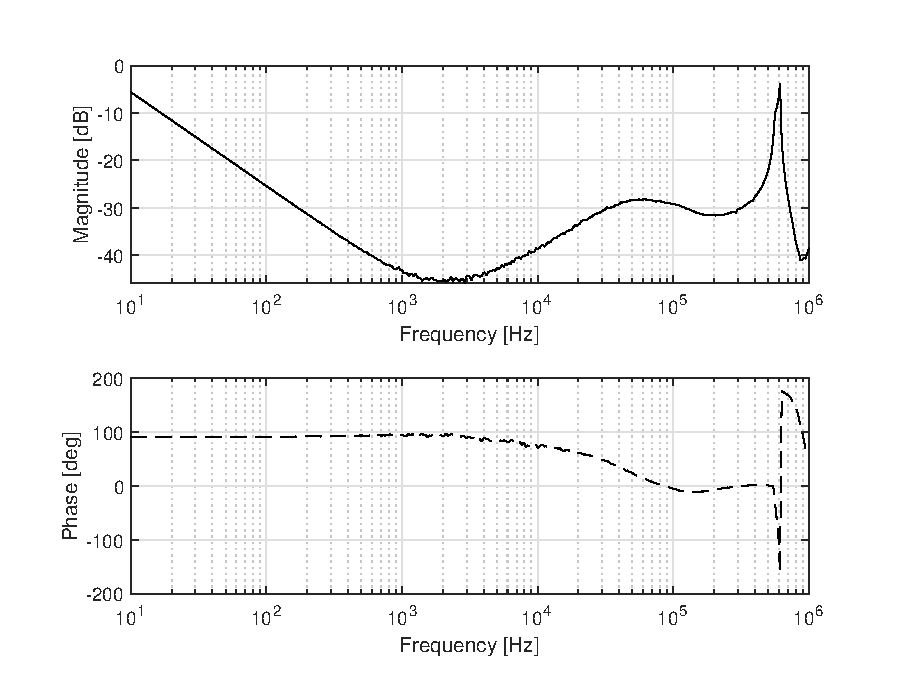
\includegraphics[width=0.6\textwidth]{Analysis/bode100_measurement_pi_open_lqr_closed.eps}
%	\caption{Measurement of frequency response of PI with closed LQR controller and $R_{\mathrm{BTL}}=\SI{4}{\ohm}$}
%	\label{fig:bode100_measurement_pi_open_lqr_closed}
%\end{figure}

\begin{figure}[H]
	\centering
	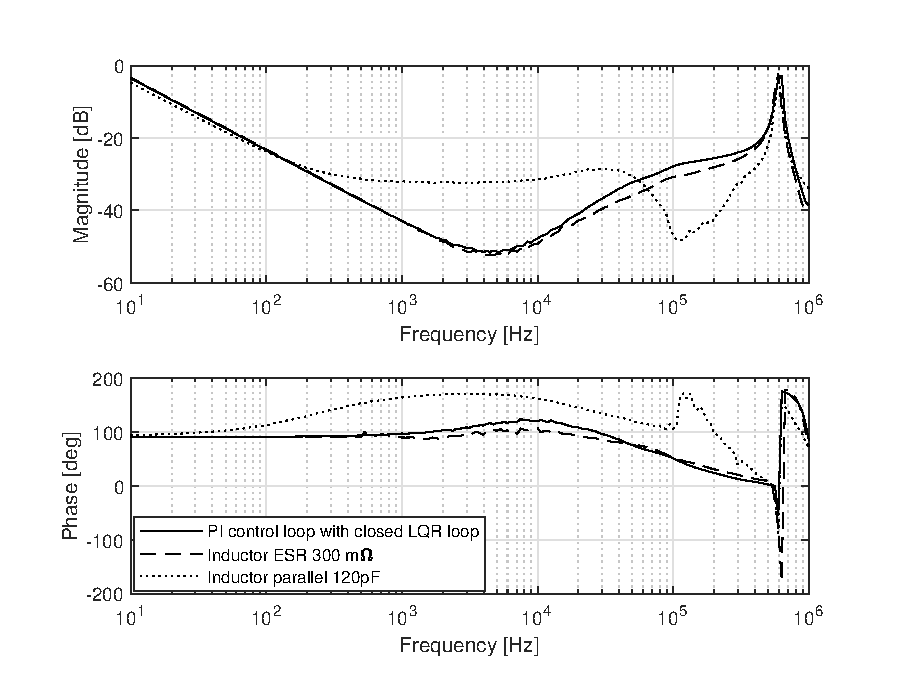
\includegraphics[width=0.8\textwidth]{Analysis/bode100_tf_pi_lqr_closed_300mohm_120pf.eps}
	\caption{Measurement of frequency response of PI with closed LQR controller with addition of parasitic elements}
	\label{fig:bode100_measurement_pi_open_lqr_closed_esr}
\end{figure}
Seen in \autoref{fig:bode100_measurement_pi_open_lqr_closed_esr} are bode plots displaying the change in magnitude and phase response with addition of parasitic elements in the filter inductor. 

\subsection{Outer loop open, inner loop open}
Next the inner loop (LQR) will be opened and only the PI controller will remain loop under test. The same measurements will be repeated and discussed.

\begin{figure}[H]
	\centering
	

\tikzset{every picture/.style={line width=0.75pt}} %set default line width to 0.75pt        

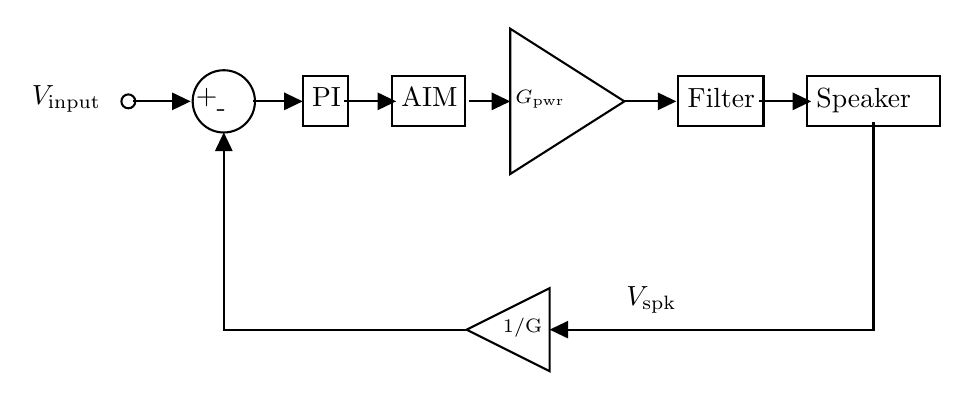
\begin{tikzpicture}[x=0.75pt,y=0.75pt,yscale=-1,xscale=1]
%uncomment if require: \path (0,888); %set diagram left start at 0, and has height of 888

%Shape: Triangle [id:dp7532010602447068] 
\draw   (298,45) -- (243,80) -- (243,10) -- cycle ;

%Shape: Triangle [id:dp15332581012771063] 
\draw   (222,155) -- (262,135) -- (262,175) -- cycle ;
%Straight Lines [id:da5523748626192453] 
\draw    (119,45) -- (140,45) ;
\draw [shift={(143,45)}, rotate = 180] [fill={rgb, 255:red, 0; green, 0; blue, 0 }  ][line width=0.08]  [draw opacity=0] (8.93,-4.29) -- (0,0) -- (8.93,4.29) -- cycle    ;
%Straight Lines [id:da3339718462186836] 
\draw    (163,45) -- (185,45) ;
\draw [shift={(188,45)}, rotate = 180] [fill={rgb, 255:red, 0; green, 0; blue, 0 }  ][line width=0.08]  [draw opacity=0] (8.93,-4.29) -- (0,0) -- (8.93,4.29) -- cycle    ;
%Straight Lines [id:da31791499009589597] 
\draw    (223,45) -- (240,45) ;
\draw [shift={(243,45)}, rotate = 180] [fill={rgb, 255:red, 0; green, 0; blue, 0 }  ][line width=0.08]  [draw opacity=0] (8.93,-4.29) -- (0,0) -- (8.93,4.29) -- cycle    ;
%Straight Lines [id:da5170788170117406] 
\draw    (298,45) -- (320,45) ;
\draw [shift={(323,45)}, rotate = 180] [fill={rgb, 255:red, 0; green, 0; blue, 0 }  ][line width=0.08]  [draw opacity=0] (8.93,-4.29) -- (0,0) -- (8.93,4.29) -- cycle    ;
%Straight Lines [id:da8953286633069386] 
\draw    (363,45) -- (385,45) ;
\draw [shift={(388,45)}, rotate = 180] [fill={rgb, 255:red, 0; green, 0; blue, 0 }  ][line width=0.08]  [draw opacity=0] (8.93,-4.29) -- (0,0) -- (8.93,4.29) -- cycle    ;
%Straight Lines [id:da8861023692104835] 
\draw    (418,55) -- (418,155) -- (265,155) ;
\draw [shift={(262,155)}, rotate = 360] [fill={rgb, 255:red, 0; green, 0; blue, 0 }  ][line width=0.08]  [draw opacity=0] (8.93,-4.29) -- (0,0) -- (8.93,4.29) -- cycle    ;
%Straight Lines [id:da16951160745617155] 
\draw    (222,155) -- (105,155) -- (105,63) ;
\draw [shift={(105,60)}, rotate = 450] [fill={rgb, 255:red, 0; green, 0; blue, 0 }  ][line width=0.08]  [draw opacity=0] (8.93,-4.29) -- (0,0) -- (8.93,4.29) -- cycle    ;
%Straight Lines [id:da9897349414536416] 
\draw    (61.35,45) -- (86,45) ;
\draw [shift={(89,45)}, rotate = 180] [fill={rgb, 255:red, 0; green, 0; blue, 0 }  ][line width=0.08]  [draw opacity=0] (8.93,-4.29) -- (0,0) -- (8.93,4.29) -- cycle    ;
\draw [shift={(59,45)}, rotate = 0] [color={rgb, 255:red, 0; green, 0; blue, 0 }  ][line width=0.75]      (0, 0) circle [x radius= 3.35, y radius= 3.35]   ;
%Shape: Circle [id:dp16935813826192136] 
\draw   (90,45) .. controls (90,36.72) and (96.72,30) .. (105,30) .. controls (113.28,30) and (120,36.72) .. (120,45) .. controls (120,53.28) and (113.28,60) .. (105,60) .. controls (96.72,60) and (90,53.28) .. (90,45) -- cycle ;


% Text Node
\draw    (143,33) -- (165,33) -- (165,57) -- (143,57) -- cycle  ;
\draw (146,37) node [anchor=north west][inner sep=0.75pt]   [align=left] {PI};
% Text Node
\draw    (186,33) -- (221,33) -- (221,57) -- (186,57) -- cycle  ;
\draw (189,37) node [anchor=north west][inner sep=0.75pt]   [align=left] {AIM};
% Text Node
\draw    (324,33) -- (365,33) -- (365,57) -- (324,57) -- cycle  ;
\draw (327,37) node [anchor=north west][inner sep=0.75pt]   [align=left] {Filter};
% Text Node
\draw    (386,33) -- (450,33) -- (450,57) -- (386,57) -- cycle  ;
\draw (389,37) node [anchor=north west][inner sep=0.75pt]   [align=left] {Speaker};
% Text Node
\draw (238,148) node [anchor=north west][inner sep=0.75pt]  [font=\scriptsize] [align=left] {1/G};
% Text Node
\draw (311,140.5) node   [align=left] {$V_{\mathrm{spk}}$};
% Text Node
\draw (11,36) node [anchor=north west][inner sep=0.75pt]   [align=left] {$V_{\mathrm{input}}$};
% Text Node
\draw (100,45) node [anchor=north west][inner sep=0.75pt]   [align=left] {\mbox{-}};
% Text Node
\draw (90,37) node [anchor=north west][inner sep=0.75pt]   [align=left] {+};
% Text Node
\draw (244,38) node [anchor=north west][inner sep=0.75pt]  [font=\scriptsize] [align=left] {$G_{\mathrm{pwr}}$};


\end{tikzpicture}

	\caption{Diagram of PI controller feedback loop}
	\label{fig:control_diagram_pi_controller}
\end{figure}
Seen in \autoref{fig:control_diagram_pi_controller} is the control loop with only the outer feedback loop active. The same parameters in the test will be repeated and measured. 
\subsubsection{Parasitic elements}
\begin{figure}[H]
	\centering
	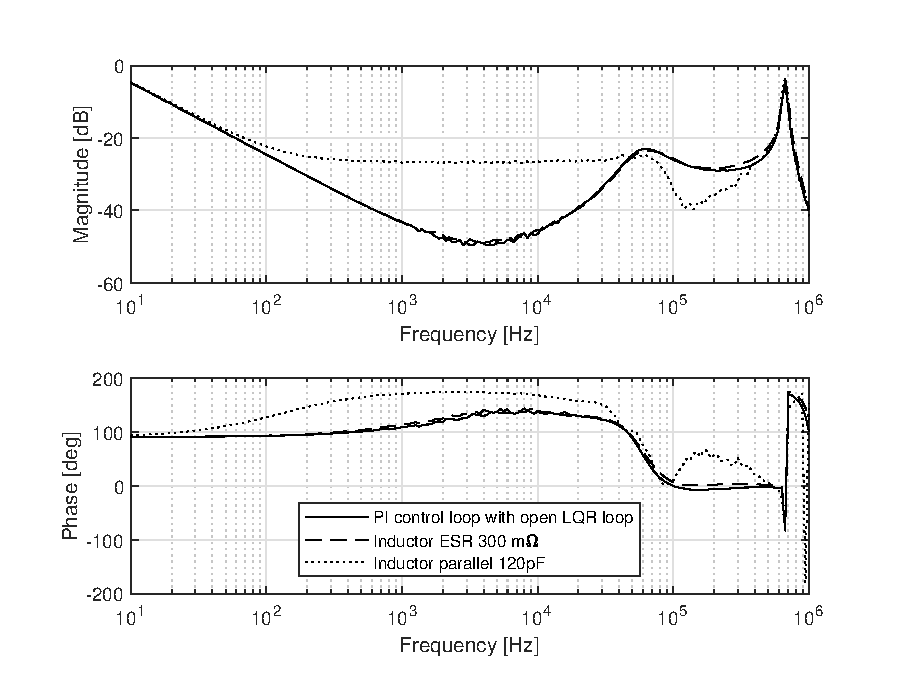
\includegraphics[width=0.8\textwidth]{Analysis/bode100_tf_pi_lqr_open_300mohm_120pf.eps}
	\caption{Measurement of frequency response of PI with open LQR controller with addition of parasitic elements}
	\label{fig:bode100_measurement_pi_open_lqr_open_esr}
\end{figure}

In \autoref{fig:bode100_measurement_pi_open_lqr_open_esr} is the frequency response of the outer control loop with the inner loop open.

\subsection{Discussion}
In this discussion section, the data collected from control loop measurements in the two parameterised tests will be processed using \autoref{lst:bode100importer.m}. Using System Identification Toolbox \cite{matlab_sysident_toolbox} a transfer function can be estimated to create dynamic system models from measured data. 

Looking at the addition of the series resistance of the inductor there is no significant change in the frequency response. Only with the addition of a parallel capacitance the frequency band between \SIrange{1}{50}{\kilo\hertz} is changed seemingly with an addition of a zero around \SI{300}{\hertz}. This is expected as per the analytical investigation into the effect of the output filter transfer function with the addition of a parallel capacitor from \Cref{eq:tf_outputfilter_reduction,eq:tf_outputfilter_esr_reduction,eq:tf_outputfilter_parallel_c_reduction}.

The preliminary indication looking at the measured transfer functions \Cref{fig:bode100_measurement_pi_open_lqr_closed_esr,fig:bode100_measurement_pi_open_lqr_open_esr} indicates the closed versus open of the LQR loop is not significantly affected by the addition of inductor parasitic elements in the low frequency band. In other words, closing the LQR loop had no mitigating effects on the parasitic elements influence on the parasitic elements. It did, however, did mitigate a discontinuity in the frequency band between \SIrange[scientific-notation = engineering]{100}{500}{\kilo\hertz} range both in the magnitude response and phase delay. This does not seem to be exclusively related to the parasitic elements introduced during the measurements, as the control loop without any added parasitic elements is also displays this characteristic.

\begin{figure}[htbp]
	\centering
	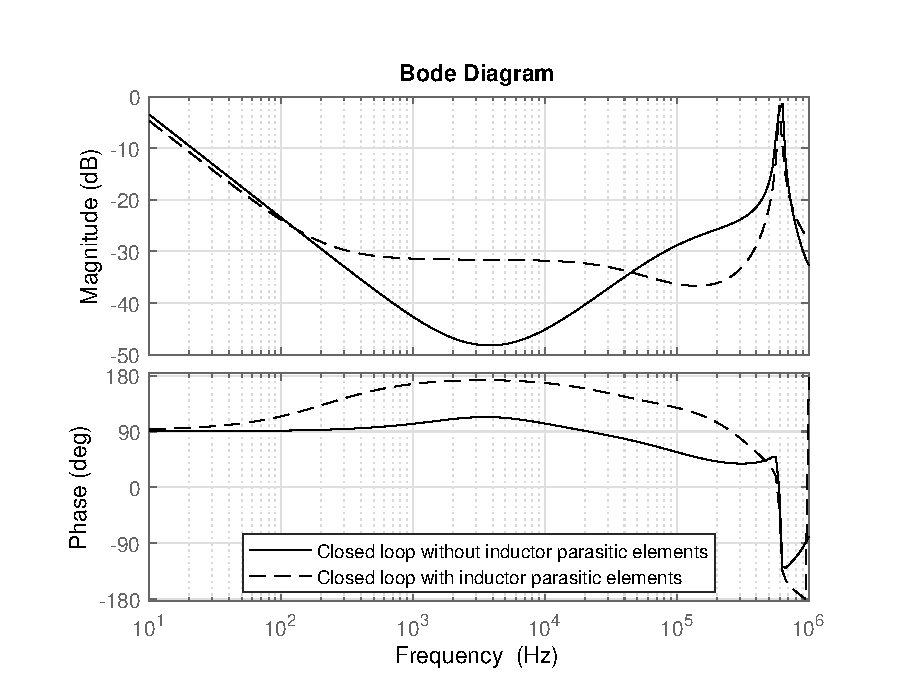
\includegraphics[width=0.8\textwidth]{Analysis/bode100_estimated_tf.eps}
	\caption{Estimated transfer functions of PI loop with closed LQR loop}
	\label{fig:bode100_estimated_tf}
\end{figure}
In \autoref{fig:bode100_estimated_tf} is the estimated control loop transfer functions using fourth-order transfer function estimation. It appears that the modulation frequency peak at \SI{600}{\kilo\hertz} has been shifted up in frequency to \SI{4}{\mega\hertz} as the transfer function was estimated. This is a processing artifact but is not part of the measurement. Plausibly the estimation error could be mitigated by applying the transfer function estimation with a higher order. However, this is deemed not of significance for the parasitic element transfer function analysis.

\begin{figure}[htbp]
	\centering
	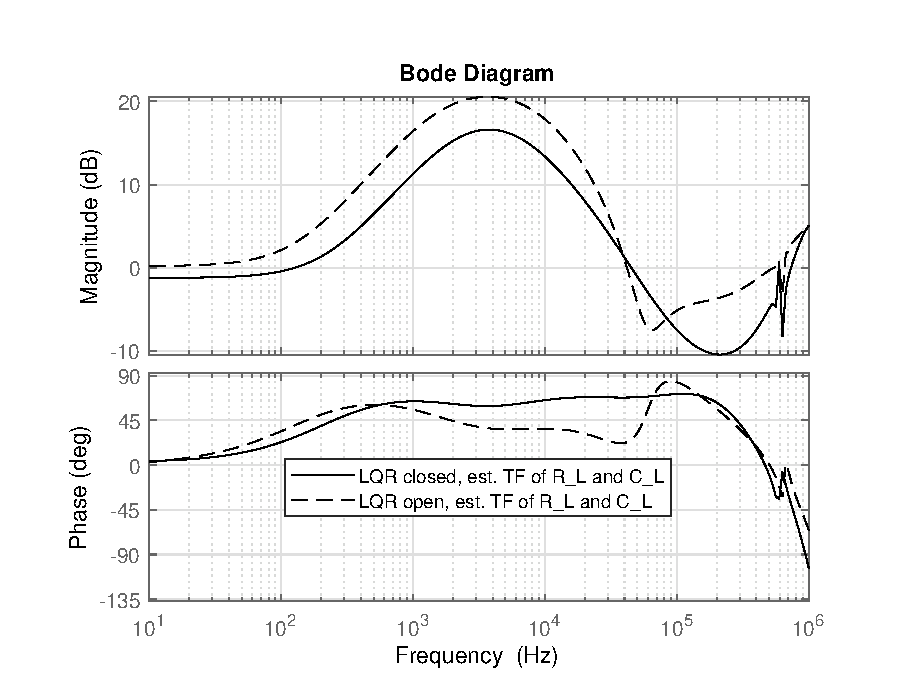
\includegraphics[width=0.8\textwidth]{Analysis/bode100_estimated_parasitic_transfer_function.eps}
	\caption{Estimation of transfer function of inductor parasitic elements on PI loop with and without LQR loop based on \autoref{fig:bode100_estimated_tf}}
	\label{fig:bode100_estimated_parasitic_transfer_function}
\end{figure}
In \autoref{fig:bode100_estimated_parasitic_transfer_function} the transfer function of the inductor parasitic elements are estimated with a division calculation in MATLAB. As the transfer function is calculated with a function division it produces a relative transfer function to determine the frequency bands that are most affected by the parasitic elements. It is noted that particularly in the frequency band between \SIrange[scientific-notation = engineering]{10}{100}{\kilo\hertz} the parasitic elements add a significant gain of \SI{15}{\decibel} and approximately \ang{45} of phase shift. 

As the PI control loop has a time constant $\tau_{i} = \SI{50}{\micro\second}$ and the effect of the parasitic transfer function in the higher frequencies at \SI{100}{\kilo\hertz} is in an interval of \SI{10}{\micro\second} it is proposed to change the PI controller time constant $\tau_{i}$ to an order of five times larger. This would mean adjusting the value of the PI controller resistor $R_{\mathrm{PI}}$ from \SI{33}{\kilo\ohm} to \SI{6.6}{\kilo\ohm}. This would mean a more aggressive integrator with a time constant of \SI{9.9}{\micro\second}.
\subsubsection{Theoretical control loop}

\begin{figure}[htbp]
	\centering
	

\tikzset{every picture/.style={line width=0.75pt}} %set default line width to 0.75pt        

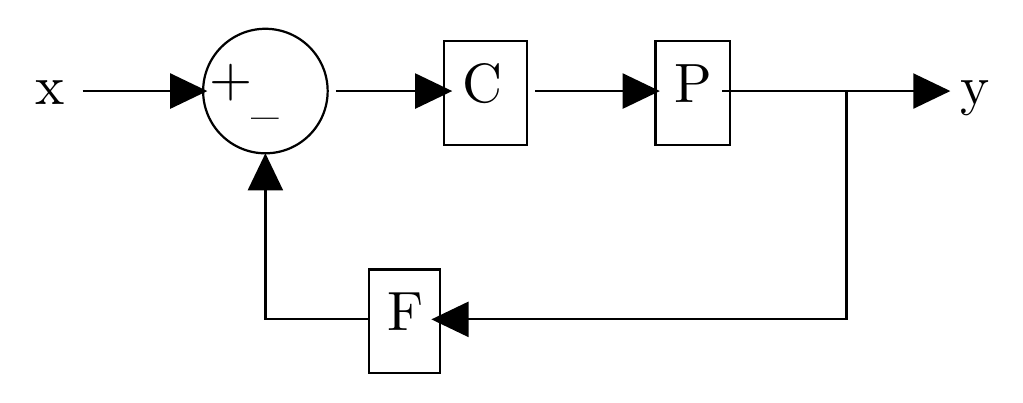
\begin{tikzpicture}[x=0.75pt,y=0.75pt,yscale=-1,xscale=1, thick, scale=2.0, every node/.style={scale=2.0}]
%uncomment if require: \path (0,101); %set diagram left start at 0, and has height of 101

%Straight Lines [id:da5523748626192453] 
\draw    (80,19) -- (105,19) ;
\draw [shift={(108,19)}, rotate = 180] [fill={rgb, 255:red, 0; green, 0; blue, 0 }  ][line width=0.08]  [draw opacity=0] (8.93,-4.29) -- (0,0) -- (8.93,4.29) -- cycle    ;
%Straight Lines [id:da3339718462186836] 
\draw    (128,19) -- (155,19) ;
\draw [shift={(158,19)}, rotate = 180] [fill={rgb, 255:red, 0; green, 0; blue, 0 }  ][line width=0.08]  [draw opacity=0] (8.93,-4.29) -- (0,0) -- (8.93,4.29) -- cycle    ;
%Straight Lines [id:da8953286633069386] 
\draw    (173,19) -- (225,19) ;
\draw [shift={(228,19)}, rotate = 180] [fill={rgb, 255:red, 0; green, 0; blue, 0 }  ][line width=0.08]  [draw opacity=0] (8.93,-4.29) -- (0,0) -- (8.93,4.29) -- cycle    ;
%Straight Lines [id:da8861023692104835] 
\draw    (203,19) -- (203,74) -- (106,74) ;
\draw [shift={(103,74)}, rotate = 360] [fill={rgb, 255:red, 0; green, 0; blue, 0 }  ][line width=0.08]  [draw opacity=0] (8.93,-4.29) -- (0,0) -- (8.93,4.29) -- cycle    ;
%Straight Lines [id:da16951160745617155] 
\draw    (88,74) -- (63,74) -- (63,37) ;
\draw [shift={(63,34)}, rotate = 450] [fill={rgb, 255:red, 0; green, 0; blue, 0 }  ][line width=0.08]  [draw opacity=0] (8.93,-4.29) -- (0,0) -- (8.93,4.29) -- cycle    ;
%Straight Lines [id:da9897349414536416] 
\draw    (19,19) -- (46,19) ;
\draw [shift={(49,19)}, rotate = 180] [fill={rgb, 255:red, 0; green, 0; blue, 0 }  ][line width=0.08]  [draw opacity=0] (8.93,-4.29) -- (0,0) -- (8.93,4.29) -- cycle    ;
%Shape: Circle [id:dp16935813826192136] 
\draw   (48,19) .. controls (48,10.72) and (54.72,4) .. (63,4) .. controls (71.28,4) and (78,10.72) .. (78,19) .. controls (78,27.28) and (71.28,34) .. (63,34) .. controls (54.72,34) and (48,27.28) .. (48,19) -- cycle ;


% Text Node
\draw    (106,7) -- (126,7) -- (126,32) -- (106,32) -- cycle  ;
\draw (109,11) node [anchor=north west][inner sep=0.75pt]   [align=left] {$\mathrm{C}$};
% Text Node
\draw    (157,7) -- (175,7) -- (175,32) -- (157,32) -- cycle  ;
\draw (160,11) node [anchor=north west][inner sep=0.75pt]   [align=left] {$\mathrm{P}$};
% Text Node
\draw (6,15) node [anchor=north west][inner sep=0.75pt]   [align=left] {$\mathrm{x}$};
% Text Node
\draw (58,22) node [anchor=north west][inner sep=0.75pt]   [align=left] {\mbox{--}};
% Text Node
\draw (48,11) node [anchor=north west][inner sep=0.75pt]   [align=left] {+};
% Text Node
\draw    (88,62) -- (105,62) -- (105,87) -- (88,87) -- cycle  ;
\draw (91,66) node [anchor=north west][inner sep=0.75pt]   [align=left] {$\mathrm{F}$};
% Text Node
\draw (229,15) node [anchor=north west][inner sep=0.75pt]   [align=left] {$\mathrm{y}$};
% Text Node
%\draw (0,30) node [anchor=north west][inner sep=0.75pt]   [align=left] {C: Control\\P: Plant\\F: Feedback};

\end{tikzpicture}

	\caption{Diagram of theoretical control loop}
	\label{fig:diagram_control_loop_theoretical}
\end{figure}

In \autoref{fig:diagram_control_loop_theoretical} the control loop is seen in its theoretical form, where $\mathrm{C}$ is control, $\mathrm{P}$ is plant, $\mathrm{F}$ is feedback and $\mathrm{x}$ and $\mathrm{y}$ are the input and output, respectively. 
When assessing the transfer function for open loop, starting on the right and moving left gives:
\begin{equation} \label{eq:control_loop_open}
	H_{o} = P \cdot C \cdot F
\end{equation}
And for the closed loop is starting on the right and moving left gives:
\begin{equation} \label{eq:control_loop_closed}
	y = P \cdot C \cdot \left( x - F \cdot y \right) 
\end{equation}
Where $C \cdot P$ is the feed-forward and $\left( x - F \cdot y \right) $ is the feedback. Applying control loop theory from \autoref{eq:control_loop_open} in the open loop to generating a theoretical transfer function of the system. This is accomplished using MATLAB and Simulink with the Control System Toolbox \cite{matlab_control_toolbox} with the simulation model in \autoref{fig:simulink_control_loop} is used to construct an open loop transfer function of the amplifier.

\begin{figure}[htbp]
	\centering
	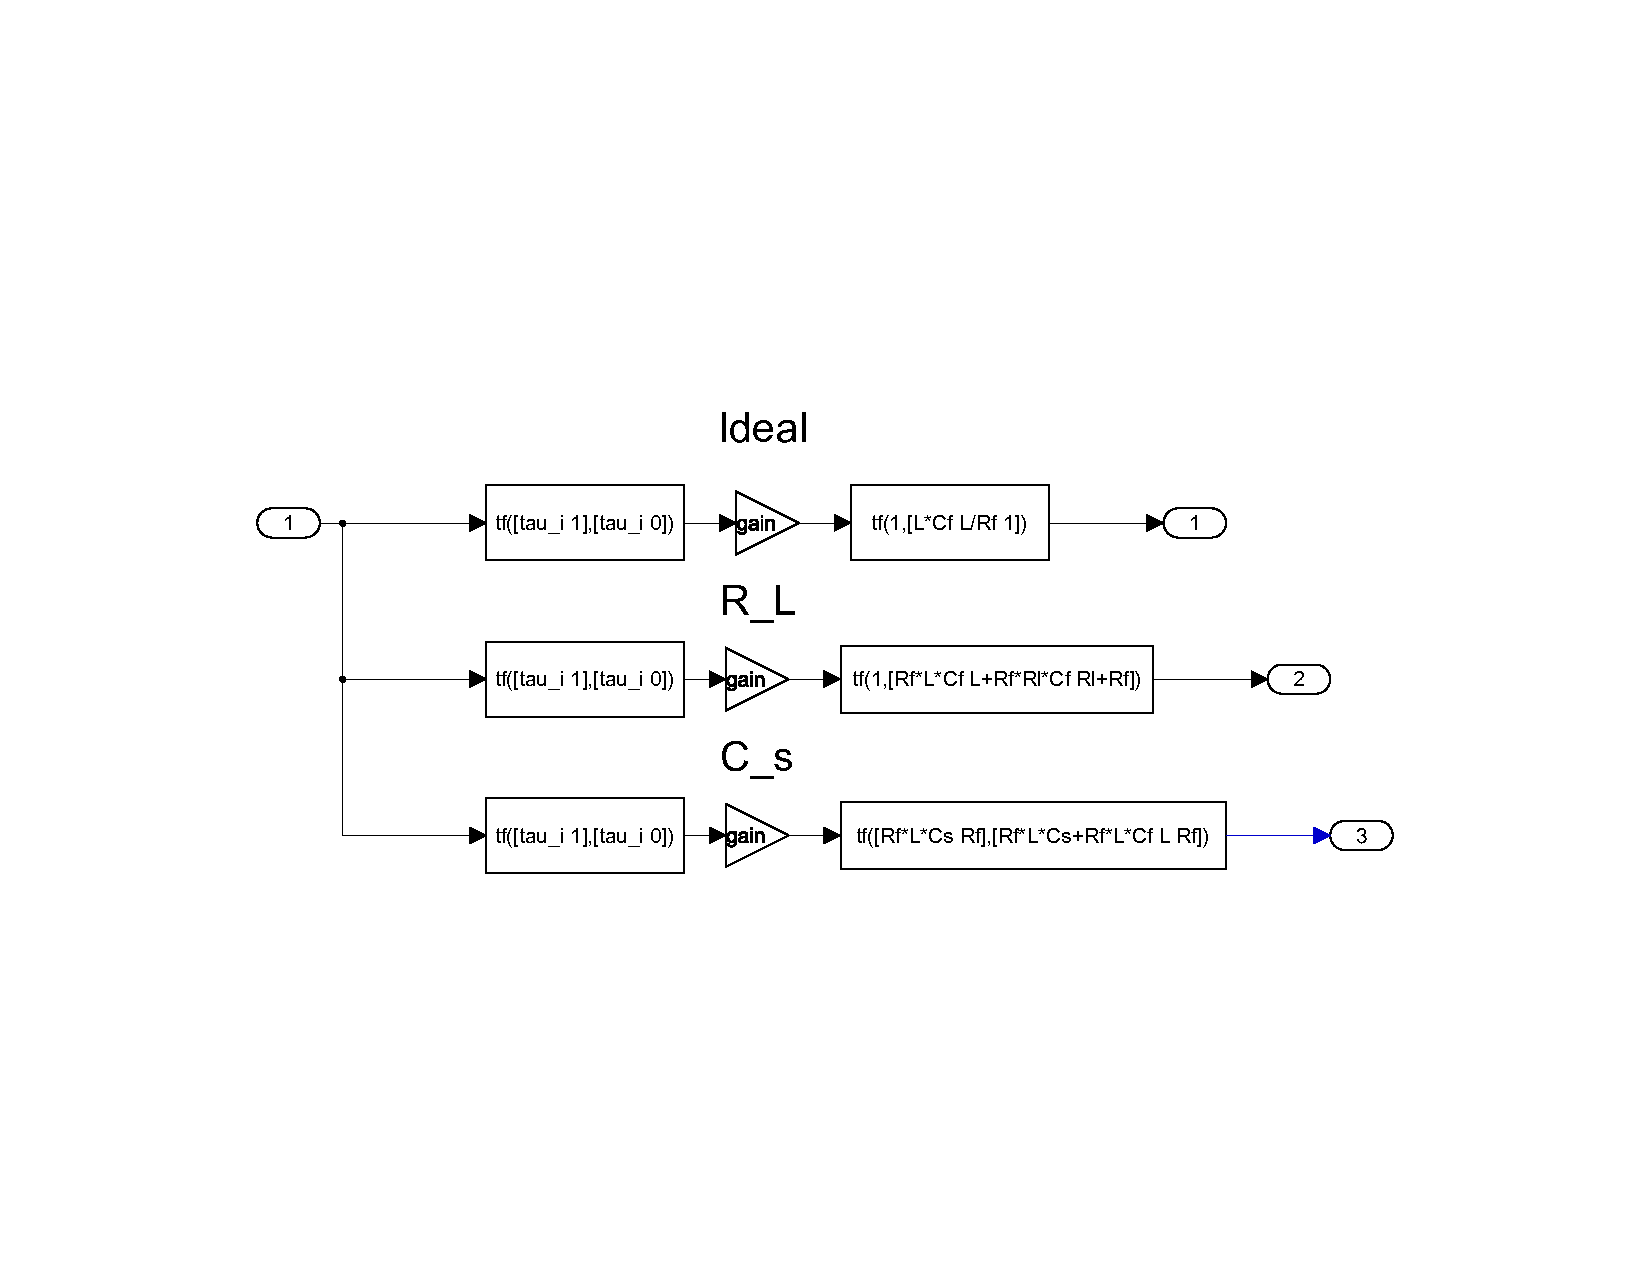
\includegraphics[width=0.8\textwidth, trim=120 180 120 180, clip]{Analysis/control_loop.pdf}
	\caption{Simulink model of open loop transfer function in control loop}
	\label{fig:simulink_control_loop}
\end{figure}

Using this Simulink model and the derived expressions from the output filter \Cref{eq:tf_outputfilter_reduction,eq:tf_outputfilter_esr_reduction,eq:tf_outputfilter_parallel_c_reduction} the open loop frequency response can be obtained.

\begin{figure}[htbp]
	\centering
	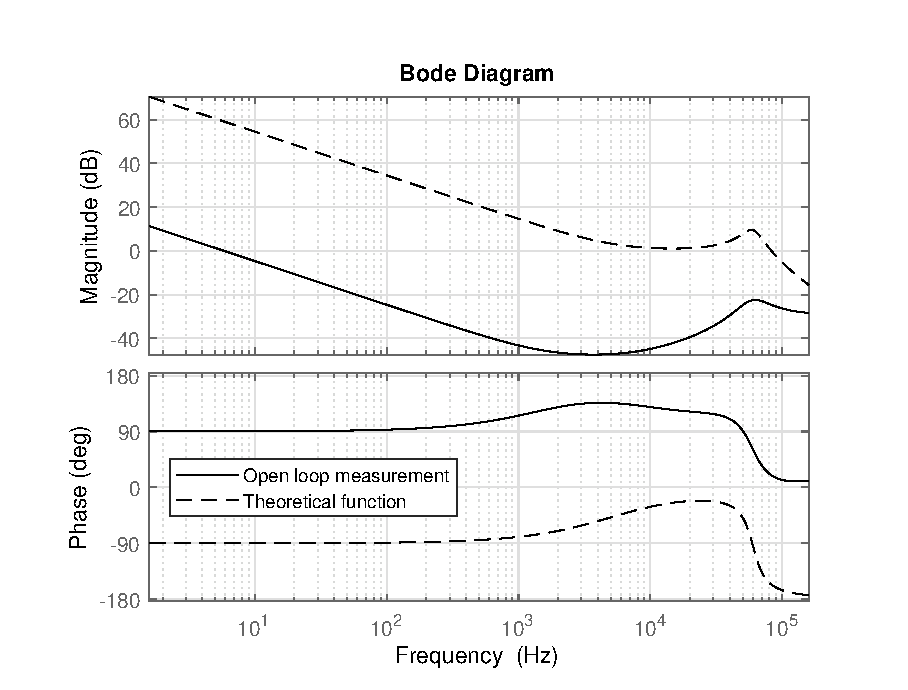
\includegraphics[width=0.8\textwidth]{Analysis/simulink_control_loop_measurement_comparison.eps}
	\caption{Comparison of measured transfer function and the theoretically obtained open loop transfer function of the system}
	\label{fig:control_loop_measurement_comparison}
\end{figure}

Seen in \autoref{fig:control_loop_measurement_comparison} is the comparison between the measured control loop using the transformer injection method and estimated with an 8th order transfer function compared with the theoretically derived expression. The increased order in the transfer function was necessary to do to obtain a meaningful comparison with the theoretical transfer function. For the purpose of validating the measurement, it seems to fit reasonably with the results that could be expected. It would appear that the measured control loop seems lower in magnitude than the actual expected transfer function level, although this could be explained when the reference level of the measuring instrument was set quite low to protect the injection transformer from overloading. This could possibly explain why there is a discrepancy in the magnitude. The difference in phase reference is probably occurred through data processing with phase wrapping performed in the analysis software.